\section{The Hales--Jewett Theorem}

Van der Waerden's theorem is about progressions in the integers. The Hales--Jewett theorem strips the arithmetic away and keeps only the combinatorics of the colour-focusing argument, and it is the stronger result: at the end of this section it will give van der Waerden's theorem back, and other things with it.

\subsection{Combinatorial Lines}

Combinatorial lines are what Hales--Jewett replaces arithmetic progressions with, and the hypercube $[n]^d$---the set of strings of length $d$ over the alphabet $[n]$---is where they live.

% [FILLED] definition supplied; the lecture used ``line'' without defining it, and the arguments below need the template
\begin{boxdefinition}[Combinatorial Line]
    Fix $n, d \in \N$ and a symbol $x \notin [n]$. A \textbf{template} is a string $\sigma \in \parenth{[n] \cup \set{x}}^d \setminus [n]^d$, ie, one in which $x$ occurs at least once; the coordinates at which $\sigma$ is $x$ are its \textbf{active coordinates}, and the others are \textbf{fixed}. For $i \in [n]$, write $\sigma(i) \in [n]^d$ for the string obtained from $\sigma$ by replacing every $x$ by $i$. The \textbf{combinatorial line} with template $\sigma$ is
    \begin{align*}
        L_\sigma = \set{\sigma(1), \sigma(2), \ldots, \sigma(n)}
    \end{align*}
    and $\sigma(n)$ is its \textbf{last point}. We will usually just say \textbf{line}.
\end{boxdefinition}

In $[3]^2$, for instance, the templates $x1$, $2x$ and $xx$ give two lines parallel to the axes and the main diagonal, whereas the anti-diagonal $\set{13, 22, 31}$ is a line in the geometric sense but not a combinatorial one, since its two coordinates move in opposite directions. The number we are after is the dimension that forces a monochromatic line.

\begin{boxdefinition}[Hales-Jewett Number]
    For all $n, r \in \N$, define $\HJ(n, r)$ to be the smallest number $d$ such that any $r$-colouring of the hypercube $[n]^d$ has a monochromatic line.
\end{boxdefinition}

As with van der Waerden's numbers, we will eventually show that these always exist.

\begin{boxtheorem}[Hales--Jewett Theorem] \label{Ch6:Thm:Hales_Jewett}
    For all $n, r \in \N$, $\HJ(n, r)$ exists.
\end{boxtheorem}

\subsection{Colour-Focused Lines}

Colour-focusing works for lines exactly as it did for arithmetic progressions.

\begin{boxdefinition}[Colour-Focused Lines]
    Given combinatorial lines $L_1, L_2, \ldots, L_s$, they are \textbf{colour-focused} if their last points coincide and each is monochromatic (in a distinct colour) on all but the last point.
\end{boxdefinition}

For example, draw $[3]^2$ as a grid, with the first coordinate running left to right and the second bottom to top. In the colouring below, the top row, the right-hand column and the diagonal are three colour-focused lines: each is monochromatic on its first two points, in orange, purple and green respectively, and all three end at the top-right point, which is their focus. Whatever colour that point gets, it completes one of them; here it is orange, and the top row is a monochromatic line.

\begin{figure}[H]
    \centering
    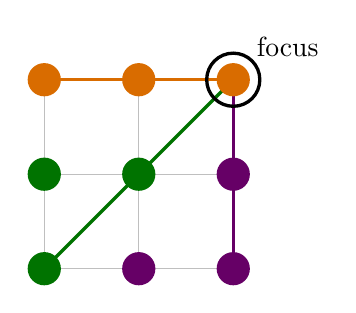
\begin{tikzpicture}[scale = 1.2]
        \draw[gray!50] (1, 1) grid (3, 3);
        \draw[orange!85!black, very thick] (1, 3) -- (3, 3);
        \draw[violet!80!black, very thick] (3, 1) -- (3, 3);
        \draw[green!45!black, very thick] (1, 1) -- (3, 3);
        \foreach \x/\y/\c in {1/3/orange!85!black, 2/3/orange!85!black, 3/3/orange!85!black, 1/2/green!45!black, 2/2/green!45!black, 3/2/violet!80!black, 1/1/green!45!black, 2/1/violet!80!black, 3/1/violet!80!black}{
            \fill[\c] (\x, \y) circle (5pt);
        }
        \draw[black, very thick] (3, 3) circle (8pt);
        \node[above right = 5pt] at (3, 3) {focus};
    \end{tikzpicture}
\end{figure}

\begin{boxdefinition}[Focused Hales-Jewett Number]
    $\FHJ(n, r, s)$ is the minimum $d$ such that any $r$-colouring of $[n]^d$ has $s$ colour-focused lines or a monochromatic line.
\end{boxdefinition}

We can see that
% [FILLED] the display was boxed as a lemma and the one-line proof supplied; the lecture said ``we can see that''
\begin{boxlemma} \label{Ch6:Lemma:HJ_le_FHJ}
    For all $n, r \in \N$,
    \begin{align*}
        \HJ(n, r) \le \FHJ(n, r, r)
    \end{align*}
\end{boxlemma}
\begin{proof}
    Let $d = \FHJ(n, r, r)$ and fix an $r$-colouring of $[n]^d$. If it has a monochromatic line we are done. Otherwise it has $r$ colour-focused lines, of $r$ distinct colours, with a common last point. That point has one of the $r$ colours, so it completes the line of that colour to a monochromatic one.
\end{proof}

We will also show
% [FILLED] the display was boxed as a lemma, with ``$2 \leq s \leq r$'' added so that $\FHJ(n, r, s - 1)$ makes sense (cf. the recursive bound on colour-focus numbers); the author's setup of the proof is kept and the argument completed from where it broke off
\begin{boxlemma} \label{Ch6:Lemma:FHJ_Recursion}
    For all $n, r, s \in \N$ with $2 \leq s \leq r$,
    \begin{align*}
        \FHJ(n, r, s) \le \FHJ(n, r, s - 1) + \HJ\of{n - 1, r^{n^{\FHJ(n, r, s - 1)}}}
    \end{align*}
\end{boxlemma}
\begin{proof}
For this argument, denote $\FHJ(n, r, s - 1)$ by $D_2$ and $\HJ\of{n - 1, r^{n^{\FHJ(n, r, s - 1)}}}$ by $D_1$. (The letters are apt because these are dimensions.) We show essentially that $\FHJ(n, r, s) \le D_2 + D_1$ and note that $D_1 = \HJ\of{n - 1, r^{n^{D_2}}}$.

% [CORRECTED] was: ``contains $s$ colour-focused lines.'' --- the definition of $\FHJ$ has two alternatives, and a colouring with a monochromatic line need not have $s$ colour-focused lines of distinct colours (a constant colouring has at most one)
The inequality is essentially saying ``any $r$-colouring of the $[n]^{D_1 + D_2}$ cube contains $s$ colour-focused lines or a monochromatic line.''

A point in my cube has coordinates

\begin{figure}[H]
    \centering
    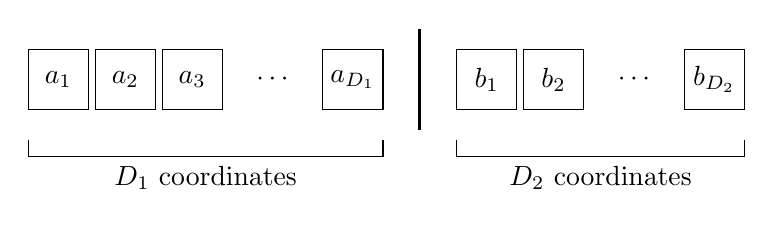
\begin{tikzpicture}[scale = 0.85]
        \foreach \x/\lab in {0/a_1, 1/a_2, 2/a_3, 4.4/a_{D_1}}{
            \draw (\x, 0) rectangle ++(0.9, 0.9);
            \node at (\x + 0.45, 0.45) {$\lab$};
        }
        \node at (3.65, 0.45) {$\cdots$};
        \draw[very thick] (5.85, -0.3) -- (5.85, 1.2);
        \foreach \x/\lab in {6.4/b_1, 7.4/b_2, 9.8/b_{D_2}}{
            \draw (\x, 0) rectangle ++(0.9, 0.9);
            \node at (\x + 0.45, 0.45) {$\lab$};
        }
        \node at (9.05, 0.45) {$\cdots$};
        \draw (0, -0.45) -- (0, -0.7) -- (5.3, -0.7) -- (5.3, -0.45);
        \node[below] at (2.65, -0.7) {$D_1$ coordinates};
        \draw (6.4, -0.45) -- (6.4, -0.7) -- (10.7, -0.7) -- (10.7, -0.45);
        \node[below] at (8.55, -0.7) {$D_2$ coordinates};
    \end{tikzpicture}
\end{figure}

I'm given a colouring of the $[n]^{D_1 + D_2}$ cube. Any string $a_1, a_2, \ldots, a_{D_1}$ completes to $n^{D_2}$ points in $[n]^{D_1 + D_2}$. Ie, there are $n^{D_2}$ ways of completing it, ie, there are $n^{D_2}$ points in $[n]^{D_1 + D_2}$ whose first $D_1$ coordinates are these. So, taken together, the $n^{D_2}$ completions of a given string can be coloured in one of $r^{n^{D_2}}$ ways, and which of these ways our colouring picks depends on the string.

In fact, we observe that \textit{any $r$-colouring of $[n]^{D_1 + D_2}$ involves an $r^{n^{D_2}}$-colouring of the $[n]^{D_1}$ cube.}

Since $D_1 = \HJ(n - 1, r^{n^{D_2}})$, there is a combinatorial line $\mathcal{L}_1 \ssq [n]^{D_1}$ whose first $n - 1$ points all get the same colour from all of the $r^{n^{D_2}}$ choices.

$\mathcal{L}_1$ corresponds to a string of the form
\begin{align*}
    \sigma \in \parenth{\brac{n - 1} \cup \set{x}}^{D_1} \setminus [n]^{D_1}
\end{align*}
(for some symbol $x$), such that the $r^{n^{D_2}}$-colouring agrees on $\sigma(1), \ldots, \sigma(n - 1)$.
% [FILLED] from here to the end of the proof: the lecture broke off at ``such that'', and the rest is supplied
Unwinding what that colouring is, this says that for all $i, i' \in [n - 1]$ and all $b \in [n]^{D_2}$, the points $\parenth{\sigma(i), b}$ and $\parenth{\sigma(i'), b}$ of our cube have the same colour. Write $\chi$ for the given $r$-colouring of $[n]^{D_1 + D_2}$, and $\chi'(b) = \chi\of{\sigma(1), b}$ for that common colour. Then $\chi'$ is an $r$-colouring of $[n]^{D_2}$, and $D_2 = \FHJ(n, r, s - 1)$, so $[n]^{D_2}$ contains a $\chi'$-monochromatic line or $s - 1$ $\chi'$-colour-focused lines.

\begin{description}
    \item[\underline{$[n]^{D_2}$ has a $\chi'$-monochromatic line $L_\tau$.}] Consider the template $\parenth{\sigma(1), \tau}$, whose active coordinates are those of $\tau$ and whose first $D_1$ coordinates are fixed at $\sigma(1)$. Its line has points $\parenth{\sigma(1), \tau(i)}$ for $i \in [n]$, of colour $\chi\of{\sigma(1), \tau(i)} = \chi'\of{\tau(i)}$, which does not depend on $i$. So $[n]^{D_1 + D_2}$ has a monochromatic line and we are done.
    \item[\underline{$[n]^{D_2}$ has $s - 1$ $\chi'$-colour-focused lines $L_{\tau_1}, \ldots, L_{\tau_{s - 1}}$.}] Let $f \in [n]^{D_2}$ be their common last point and $c_1, \ldots, c_{s - 1}$ their colours, which are distinct. If $\chi'(f) = c_j$ for some $j$, then $L_{\tau_j}$ is $\chi'$-monochromatic and the previous case applies, so suppose not. For each $j$, the template $\parenth{\sigma, \tau_j}$ has as its active coordinates those of $\sigma$ together with those of $\tau_j$, and its line has points $\parenth{\sigma(i), \tau_j(i)}$ for $i \in [n]$. For $i \leq n - 1$, the colour of such a point is $\chi\of{\sigma(i), \tau_j(i)} = \chi'\of{\tau_j(i)} = c_j$, since $\tau_j(i)$ is one of the first $n - 1$ points of $L_{\tau_j}$; and its last point is $\parenth{\sigma(n), f}$. Alongside these, the template $\parenth{\sigma, f}$, with the last $D_2$ coordinates fixed at $f$, gives a line with points $\parenth{\sigma(i), f}$, of colour $\chi\of{\sigma(i), f} = \chi'(f)$ for $i \leq n - 1$, and with the same last point $\parenth{\sigma(n), f}$. These $s$ lines are monochromatic on all but their last point, in the $s$ distinct colours $c_1, \ldots, c_{s - 1}, \chi'(f)$, and their last points coincide: they are $s$ colour-focused lines in $[n]^{D_1 + D_2}$.
\end{description}
Either way, $[n]^{D_1 + D_2}$ has a monochromatic line or $s$ colour-focused lines, so $\FHJ(n, r, s) \leq D_1 + D_2$.
\end{proof}

With the recursion in hand, the Hales--Jewett theorem goes exactly as van der Waerden's did: induct on the size of the alphabet, and inside that on the number of focused lines.

% [FILLED] the proof of the Hales--Jewett theorem is supplied: the lecture stopped at the recursion, and the theorem is what the recursion is for
\begin{proof}[Proof of \Cref{Ch6:Thm:Hales_Jewett}]
    Induct on $n$, keeping $r$ generic. When $n = 1$, the cube $[1]^1$ is a single point, which is a line (its template is $x$) and is monochromatic under any colouring, so $\HJ(1, r) = 1$.

    Now fix $n \geq 2$ and assume that $\HJ(n - 1, r')$ exists for every $r' \in \N$. By \Cref{Ch6:Lemma:HJ_le_FHJ} it suffices to show that $\FHJ(n, r, s)$ exists for all $r$ and all $1 \leq s \leq r$, which we do by induction on $s$. For $s = 1$, take $d = \HJ(n - 1, r)$: any $r$-colouring of $[n]^d$ restricts to one of $[n - 1]^d$, which has a monochromatic line with some template $\sigma \in \parenth{[n - 1] \cup \set{x}}^d$, and read in $[n]^d$ the same template gives a line whose first $n - 1$ points are that line. It is therefore monochromatic on all but its last point, which is to say that it is one colour-focused line, and so $\FHJ(n, r, 1) \leq \HJ(n - 1, r)$. For $2 \leq s \leq r$, \Cref{Ch6:Lemma:FHJ_Recursion} bounds $\FHJ(n, r, s)$ by $\FHJ(n, r, s - 1)$, which exists by the induction on $s$, plus $\HJ\of{n - 1, r^{n^{\FHJ(n, r, s - 1)}}}$, which exists by the induction on $n$.
\end{proof}

\subsection{From Lines to Progressions}

The theorem gives us a monochromatic copy of any finite pattern, in any number of colours and any dimension.

\begin{boxtheorem}
    For any finite $X \ssq \Z^k$ and any $r \in \N$, any $r$-colouring of $\Z^k$ contains a copy $\alpha X + \beta$ of $X$, for some $\alpha \in \N$ and $\beta \in \Z^k$, that is monochromatic.
\end{boxtheorem}
\begin{proof}
    % [FILLED] proof supplied, along the lines of the author's own ``IDEA'' comment: colour $[n]^d$ through the map $a \mapsto x_{a_1} + \cdots + x_{a_d}$, and read a monochromatic line off as $\alpha X + \beta$ with $\alpha$ the number of active coordinates
    Let $X = \set{x_1, \ldots, x_n} \ssq \Z^k$, so that $n = \abs{X}$, let $d = \HJ(n, r)$, which exists by \Cref{Ch6:Thm:Hales_Jewett}, and fix an $r$-colouring $\chi$ of $\Z^k$. Define
    \begin{align*}
        f : [n]^d \to \Z^k : \parenth{a_1, \ldots, a_d} \mapsto x_{a_1} + x_{a_2} + \cdots + x_{a_d}
    \end{align*}
    and give each point $a \in [n]^d$ the colour $\chi\of{f(a)}$ of its image. This is an $r$-colouring of $[n]^d$, so by the choice of $d$ it has a monochromatic line $L_\sigma$. Let $S$ be the set of active coordinates of $\sigma$ and $\alpha = \abs{S}$, so that $\alpha \geq 1$. For each $i \in [n]$, the string $\sigma(i)$ has $i$ in the $\alpha$ active coordinates and the entries of $\sigma$ itself in the rest, so
    \begin{align*}
        f\of{\sigma(i)} = \sum_{j \notin S} x_{\sigma_j} + \alpha x_i = \beta + \alpha x_i
    \end{align*}
    where $\beta = \sum_{j \notin S} x_{\sigma_j} \in \Z^k$ does not depend on $i$. Thus $f\of{L_\sigma} = \setst{\beta + \alpha x_i}{i \in [n]} = \alpha X + \beta$, and since every point of $L_\sigma$ has the same colour, so does every point of $\alpha X + \beta$ under $\chi$.
\end{proof}

This is known as Gallai's theorem, and \cite[Chapter~2]{GrahamRothschildSpencer} deduces it from the Hales--Jewett theorem of~\cite{HalesJewett} in exactly this way.

To find bounds on van der Waerden numbers in terms of Hales-Jewett numbers, let's ask ourselves the following question: can we map from $[n]^d$ to some line in a way that takes geometric/combinatorial lines to arithmetic progressions?

One thing we immediately see is that if we consider the mapping
% [CORRECTED] was: $p \mapsto p_0 + p_1 n + p_2 n^2 + \cdots + p_{d-1} n^{d-1}$ --- with coordinates in $[n] = \set{1, \ldots, n}$ that lands in $\set{\frac{n^d - 1}{n - 1}, \ldots, \frac{n^{d + 1} - n}{n - 1}}$, outside $\brac{n^d}$ once $d \geq 2$ (at $n = d = 2$ the image is $\set{3, 4, 5, 6}$); shifting each coordinate down by one gives the base-$n$ digits and a bijection onto $\brac{n^d}$, and the coordinates are indexed $1, \ldots, d$ as in $\gamma$ below
\begin{align*}
    \phi : [n]^d \to \brac{n^d} : p \mapsto 1 + \parenth{p_1 - 1} + \parenth{p_2 - 1} n + \cdots + \parenth{p_d - 1} n^{d - 1}
\end{align*}
which reads a point as the digits of a number written in base $n$, then lines go to progressions: if $S$ is the set of active coordinates of a template $\sigma$, then
\begin{align*}
    \phi\of{\sigma(i)} = 1 + \sum_{j \notin S} \parenth{\sigma_j - 1} n^{j - 1} + \parenth{i - 1} \sum_{j \in S} n^{j - 1}
\end{align*}
so as $i$ runs over $[n]$ the images $\phi\of{\sigma(1)}, \ldots, \phi\of{\sigma(n)}$ form an $n$-term arithmetic progression with common difference $\sum_{j \in S} n^{j - 1} > 0$. An $r$-colouring of $\brac{n^d}$ therefore pulls back along $\phi$ to an $r$-colouring of $[n]^d$, and when $d = \HJ(n, r)$ the monochromatic line this contains maps to a monochromatic $n$-term progression. In other words,
\begin{align*}
    \VW(n, r) \leq n^{\HJ(n, r)}
\end{align*}
so that the Hales--Jewett theorem gives van der Waerden's theorem a second time.

Nothing about this used the particular form of $\phi$ beyond one property: a line is sent to a progression that does not degenerate, because its active coordinates all move together, so the image of a line can never collapse to a point. Any map with that property gives a Ramsey theorem for whatever a line maps to.

Similarly, if we do
% [CORRECTED] was: $p \mapsto p_1^2 + p_2 ^2 + \cdots + p_d^2$ --- with coordinates in $[n]$ that takes values up to $n^2 d$, outside $\brac{(n - 1)^2 d + 1}$; the stated codomain is the one for coordinates shifted down by one, as for $\phi$
\begin{align*}
    \gamma : [n]^d \to \brac{(n - 1)^2 d + 1} : p \mapsto 1 + \parenth{p_1 - 1}^2 + \parenth{p_2 - 1}^2 + \cdots + \parenth{p_d - 1}^2
\end{align*}
the image of a line under $\gamma$ is now a ``quadratic progression''.
